\section{Results beyond Original Paper}
\jdcomment{Often papers don't include enough information to fully specify their experiments, so some additional experimentation may be necessary. For example, it might be the case that batch size was not specified, and so different batch sizes should be evaluated. Include the results of any additional experiments here. Note: this won't be necessary for all reproductions.}
 
\subsection{Sparsity Distribution vs FLOP Consumption}\label{effect-sparsity-distribution}

\begin{figure}[h]
    \centering
    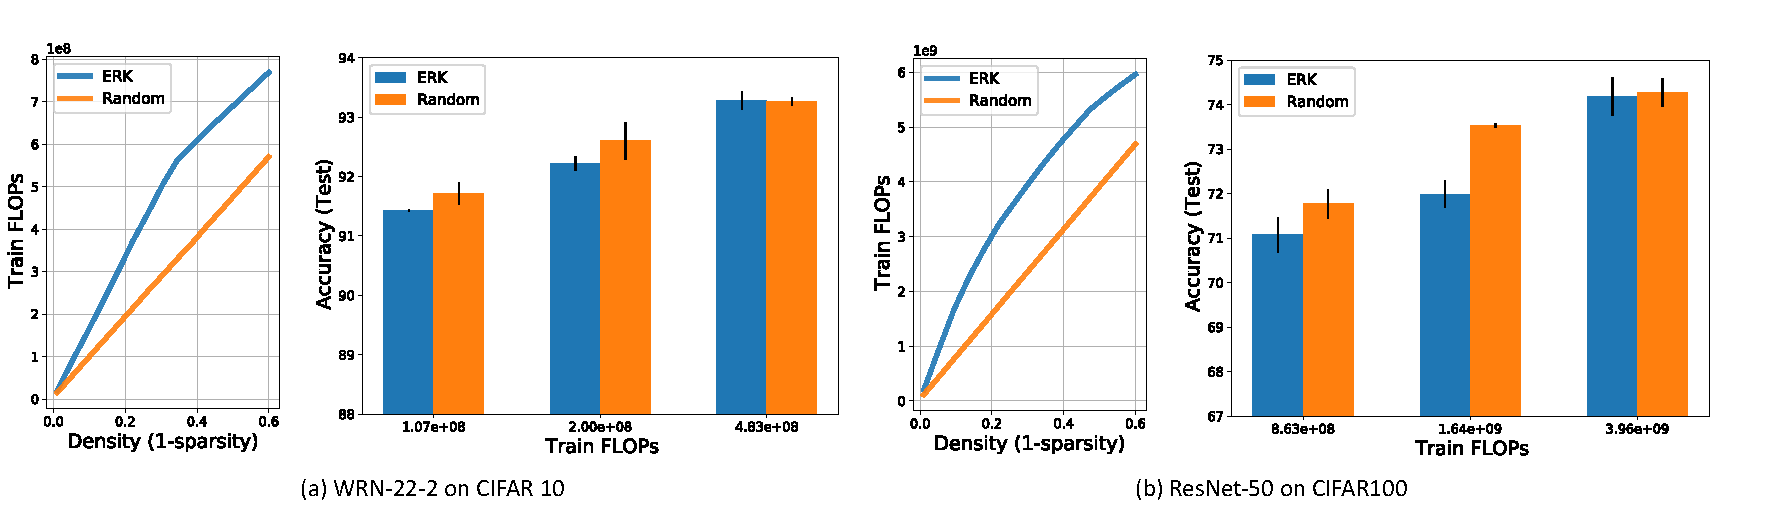
\includegraphics[width=1\textwidth]{../openreview/figs/erk_vs_random_FLOPs.pdf}
    \captionsetup{aboveskip=\figureaboveskip,belowskip=\figurebelowskip}
    \caption{\textbf{Test Accuracy vs FLOP consumption of WideResNet-22-2 on CIFAR-10 and ResNet-50 on CIFAR-100,} compared for Random and ERK initializations. For the same FLOP budget, models trained with ERK initialization must be more sparse, resulting in inferior performance.}
    \label{fig:erk-vs-random-FLOPs}
\end{figure}

While ERK initialization outperforms Random initialization consistently for a given target parameter count, it requires a higher FLOP budget. Figure \ref{fig:erk-vs-random-FLOPs} compares the two initialization schemes across fixed training FLOPs. Theoretical FLOP requirement for Random initialization scales linearly with density $(1-s)$, and is significantly lesser than ERK's FLOP requirements. Consequently, Random initialization outperforms ERK initialization for a given training budget.

\subsection{Effect of Redistribution}\label{effect-redistribution}

\begin{table}[h]
    \captionsetup{aboveskip=\tableaboveskip,belowskip=\tablebelowskip}
    \caption{\textbf{Effect of redistribution during \textit{RigL} updates, evaluated  on CIFAR10 and CIFAR100}. By utilising sparse gradient or sparse momentum based redistribution, \textit{RigL} (Random) matches \textit{RigL} (ERK)'s performance. Among Random and ERK initialized experiments, we mark the best metrics under each sparsity and dataset in bold. }
    \centering
    
    \resizebox{\textwidth}{!}{%
    \begin{tabular}{ c c cc cc cc cc}
     \toprule
    \multirow{3}{*}{\textbf{Method}} & \multirow{3}{*}{\textbf{Redistribution}} & 
    \multicolumn{4}{c}{\textbf{CIFAR-10}} & \multicolumn{4}{c}{\textbf{CIFAR-100}} \\
    \cmidrule(lr){3-6} \cmidrule(lr){7-10}
    
    {} & {} &
    \multicolumn{2}{c}{$1 - s=0.1$} & \multicolumn{2}{c}{$1 - s=0.2$} &
    \multicolumn{2}{c}{$1 - s=0.1$} & \multicolumn{2}{c}{$1 - s=0.2$} \\
    \cmidrule(lr){3-4} \cmidrule(lr){5-6} \cmidrule(lr){7-8} \cmidrule(lr){9-10}
    
    {} & {} &
    \makecell{Accuracy $\uparrow$ \\ (Test)}  & \makecell{FLOPs $\downarrow$  \\ (Train, Test)} &
    \makecell{Accuracy $\uparrow$ \\ (Test)}  & \makecell{FLOPs $\downarrow$  \\ (Train, Test)}  &
    \makecell{Accuracy $\uparrow$ \\ (Test)}  & \makecell{FLOPs $\downarrow$  \\ (Train, Test)} &
    \makecell{Accuracy $\uparrow$ \\ (Test)}  & \makecell{FLOPs $\downarrow$  \\ (Train, Test)} \\
    \midrule
    
    \multicolumn{10}{c}{Random Initialization} \\
    \midrule
    
    {RigL} & {-} &
    {91.7 $\pm$ 0.18} & {0.10x, 0.10x} &
    {92.9 $\pm$ 0.10} & {0.20x, 0.20x} &
    {71.8 $\pm$ 0.33} & {0.10x, 0.10x} &
    {73.5 $\pm$ 0.04} & {0.20x, 0.20x} \\
    
    {RigL-SG} & {Sparse Grad} &
    \textbf{92.2 $\pm$ 0.17} & {0.28x, 0.28x} &
    {92.7 $\pm$ 0.25} & {0.49x, 0.49x} &
    {72.3 $\pm$ 0.12} & {0.36x,0.35x} &
    \textbf{73.7 $\pm$ 0.15} & {0.53x, 0.53x} \\
    
    {RigL-SM} & {Sparse Mmt} &
    \textbf{92.2 $\pm$ 0.20} & {0.28x, 0.28x} &
    \textbf{92.9 $\pm$ 0.21} & {0.50x, 0.49x} &
    \textbf{72.6 $\pm$ 0.27} & {0.36x,0.36x} &
    \textbf{73.7 $\pm$ 0.35} & {0.53x, 0.53x} \\
    
    \midrule
    \multicolumn{10}{c}{ERK Initialization} \\
    \midrule
    
    {RigL} & {-} &
    \textbf{92.4 $\pm$ 0.06} & {0.17x, 0.17x} &
    \textbf{93.1 $\pm$ 0.09} & {0.35x, 0.35x} &
    {72.6 $\pm$ 0.37} & {0.23x, 0.22x} &
    {73.4 $\pm$ 0.15} & {0.38x, 0.38x} \\
    
    {RigL-SG} & {Sparse Grad} &
    {92.1 $\pm$ 0.19} & {0.28x, 0.28x} &
    {92.7 $\pm$ 0.19} & {0.49x, 0.49x} &
    \textbf{73.0 $\pm$ 0.13} & {0.37x,0.36x} &
    {74.2 $\pm$ 0.26} & {0.53x, 0.53x} \\
    
    {RigL-SM} & {Sparse Mmt} &
    \textbf{92.27 $\pm$ 0.01} & {0.28x, 0.28x} &
    \textbf{93.0 $\pm$ 0.13} & {0.50x, 0.49x} &
    {72.6 $\pm$ 0.27} & {0.37x, 0.37x} &
    \textbf{74.2 $\pm$ 0.13} & {0.53x, 0.53x} \\
    
    \midrule
    \multicolumn{10}{c}{Re-Initialization with \textit{RigL}-SM (Random, ERK)} \\
    \midrule
    
    \makecell{RigL} & {-} &
    {90.3 $\pm$ 0.34} & {0.28x, 0.28x} &
    {91.0 $\pm$ 0.38} & {0.50x, 0.49x} &
    {67.6 $\pm$ 0.28} & {0.36x, 0.36x} &
    {68.9 $\pm$ 0.65} & {0.53x, 0.53x} \\
    
    \makecell{RigL (ERK)} & {-} &
    {90.2 $\pm$ 0.57} & {0.28x, 0.28x} &
    {90.6 $\pm$ 0.56} & {0.50x, 0.49x} &
    {67.8 $\pm$ 0.73} & {0.37x, 0.37x} &
    {68.9 $\pm$ 0.47} & {0.53x, 0.53x} \\
    \bottomrule
    
    \end{tabular}%
    }
    
    \label{tab:effect-redistribution}
\end{table}

One of the main differences of \textit{RigL} over SNFS is the lack of layer-wise redistribution during training. We examine if using a redistribution criterion can be beneficial and bridge the performance gap between Random and ERK initialization. Following \citet{dettmers2020sparse}, during every mask update, we reallocate layer-wise density proportional to its average sparse gradient or momentum (\textit{RigL}-SG, \textit{RigL}-SM).\\
 
Table \ref{tab:effect-redistribution} shows that redistribution significantly improves \textit{RigL} (Random), but not \textit{RigL} (ERK). We additionally plot the FLOP requirement against training steps and the final sparsity distribution in Figure \ref{fig:density-dist-evolution}. The layer-wise sparsity distribution largely becomes constant within a few epochs. The final distribution is similar, but more ``extreme'' than ERK---wherever ERK exceeds/falls short of Random, redistribution does so by a greater extent.\\

By allocating higher densities to $1 \times 1$ convolutions (\textit{convShortcut} in Figure \ref{fig:density-dist-evolution}), redistribution significantly increases the FLOP requirement---and hence, is not a preferred alternative to ERK. Surprisingly, initializing \textit{RigL} with the final sparsity distribution in a manner similar to the Lottery Ticket Hypothesis results in subpar performance (group 3, Table \ref{tab:effect-redistribution}). 

\begin{figure}[!ht]
    \centering
    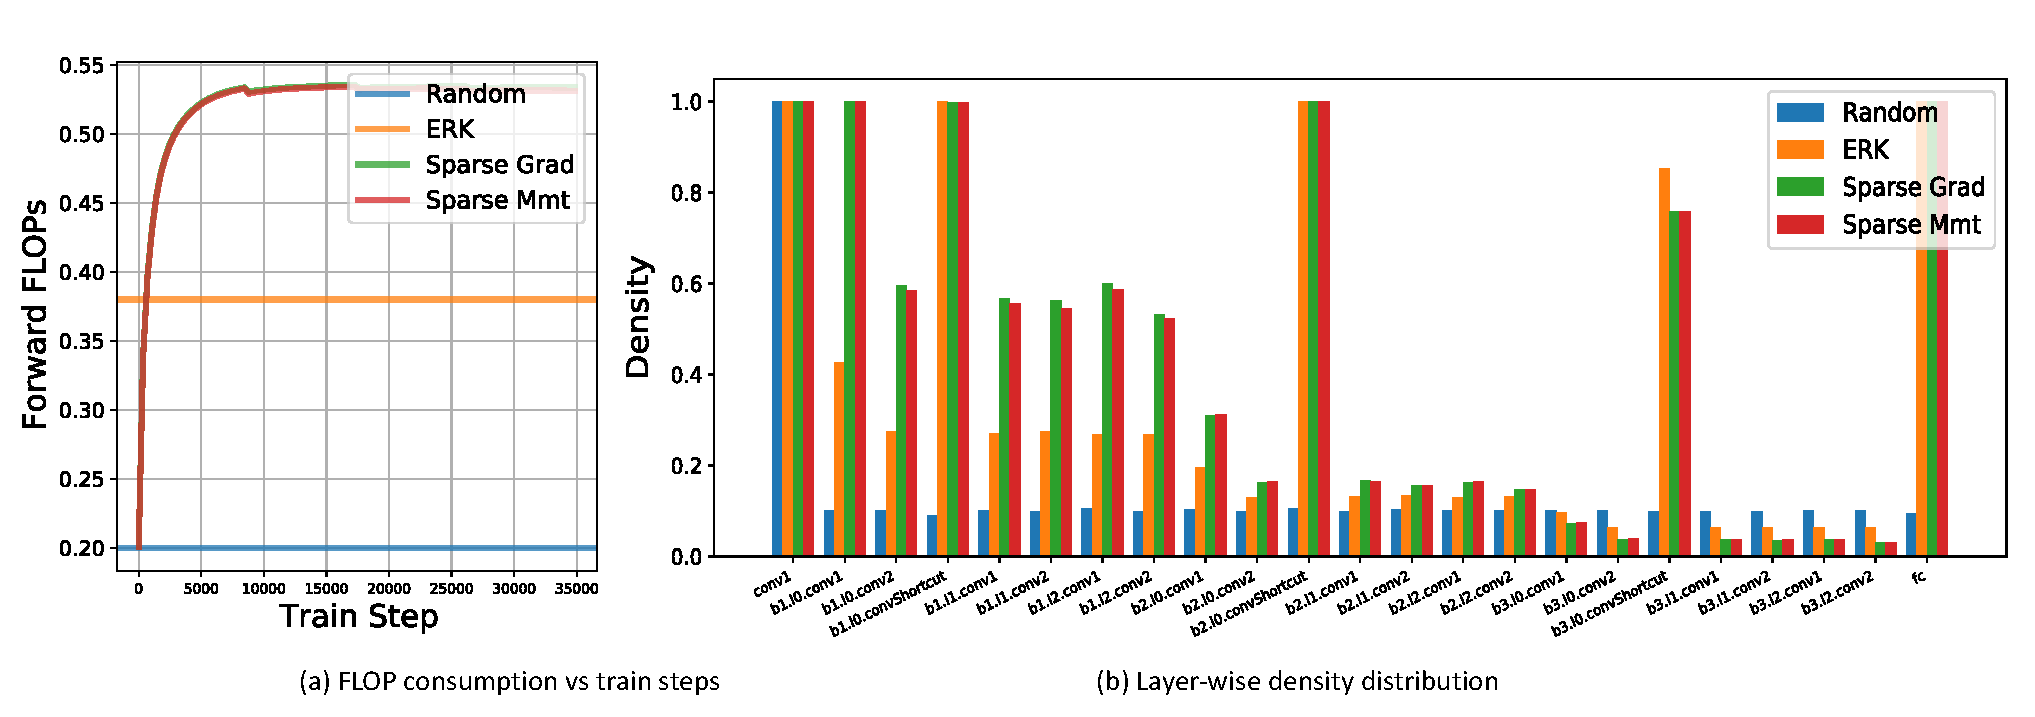
\includegraphics[width=1\textwidth]{../openreview/figs/density_dist_evolution.pdf}
    \captionsetup{aboveskip=\figureaboveskip,belowskip=\figurebelowskip}
    \caption{\textbf{Effect of redistribution on \textit{RigL}'s performance,} evaluated using WideResNet-22-2 on CIFAR10 at 80\% sparsity. \textbf{(left)} FLOPs required per forward pass, shown relative to the dense baseline, rises quickly and saturates within a few epochs (\textasciitilde10k steps) for both sparse gradient and sparse momentum based redistribution. \textbf{(right)} Comparison of the final density distribution against Random and ERK counterparts. ``b'' refers to block and ``l'' layer here.}
    \label{fig:density-dist-evolution}
\end{figure}